\chapter{Meson Spectra}
\label{ch:meson_spectra}

\begin{flushright}
If it disagrees with experiment it is wrong. In that simple statement\\
is the key to science. It does not make any difference how beautiful\\
your guess is. It does not make any difference how smart you are, who\\
made the guess, or what his name is � if it disagrees with experiment\\
it is wrong. That is all there is to it. -- Richard Feynman
\end{flushright}

In this chapter, we calculate the meson spectra for the vector, axial-vector, and pseudoscalar mesons from the dynamical three-field model of AdS/QCD introduced in the preceding chapter.
The analysis is much the same as that presented in Chapter \ref{sec:Soft-Wall-Model}.

To calculate the spectra of the radial excitations of the mesons, we examine the relevant terms from the string frame action (\ref{eqStringAction}),
\be
\cS_{{\rm meson}}=-\frac{1}{16\pi G_5} \int d^5x \sqrt{-g} e^{-2\Phi}\mathrm{Tr}\left[ \left|DX\right|^2+V_m(\Phi,X^2,\mathcal{G})+\frac{1}{2g_5^2}\left(F_A^2 +F_V^2\right) \right] \, .
\label{eqMesonL}
\ee
The $2 \times 2$ field $X$ contains the scalar and pseudoscalar fields $(S,\pi)$, as well as the VEV.
We will use the exponential representation for the scalar field discussed in \cite{bartz-pions},
\be
X_e = \left( S(x,z)+\frac{\chi(z)}{2}\right)I \, e^{2i\pi^a_e(x,z)t^a},
\ee
where $I$ is the $2\times2$ identity matrix.
The scalar potential $V_m$ does not contribute to the equations of motion for the vector, axial-vector, or pseudoscalar mesons, although terms from the background potential $U(\phi,\chi, G)$ will be useful in the pseudoscalar analysis.

\section{Vector Sector}
We find the equations of motion for the various meson fields by varying the meson action and performing a Kaluza-Klein decomposition.
For the vector sector, the equation of motion takes the following form,
\be
-\partial_{z}^{2}V_{n}+\omega'\partial_{z}V_{n}=m_{V_{n}}^{2}V_{n},
\ee
where we have again defined $\omega \equiv \Phi(z)+\log z.$
We can eliminate the first derivative of the field, bringing the equation of motion into Schr{\"o}dinger-like form, using the substitution 
\be
V_{n}(z)=e^{\omega/2}v_{n}(z).
\ee
The equation of motion is now
\be
-v_{n}^{''}+\left(\frac{1}{4}\omega^{'2}-\frac{1}{2}\omega^{''}\right)v_{n}=m_{V_{n}}^{2}v_{n}
\ee
These equations are analytically solvable in the IR limit, giving the same result found in Section \ref{sec:Soft-Wall-Model}, but full analysis requires the use of a numerical shooting method to find the mass eigenvalues.
This model finds a better phenomenological fit than the results presented in \cite{gherghetta-kelley}, particularly for the ground state $\rho$ meson, as shown in Figure \ref{figRho}. 

\begin{figure}[htb]
\center{\includegraphics[width=300pt]{rho.eps}}
\caption{Comparison of the predicted mass eigenvalues for the vector sector with the experimental $\rho$ meson spectrum \cite{PDG}.}
\label{figRho}
\end{figure}


\begin{table}[htb]
\center
\begin{tabular}{| c || c | c  |}
\hline
n & $\rho$ experimental (MeV) & $\rho$ model \\
\hline
1 & 775.5 $\pm$  1 & 860	\\
2 & 1282 $\pm$ 37 & 1216 \\
3 & 1465 $\pm$ 25 & 1489 \\
4 &  1720 $\pm$ 20 & 1720 \\ 
5 &  1909 $\pm$ 30 & 1923 \\
6 &  2149 $\pm$  17& 2107 \\
7 &  2265 $\pm$  40& 2276 \\ 
\hline
\end{tabular}
\caption{The experimental \cite{PDG} and predicted values for the masses of the vector mesons.}
\label{tabRho}
\end{table}

\section{Axial-Vector Sector}
Varying the action with respect to the axial vector field and performing a KK decomposition,the equation of motion becomes
\be
-\partial_z^2 A_{n}+\omega'\partial_zA_{n} +\frac{g_5^2 \chi(z)^2}{z^2}= m_{A_{n}}^{2}A_{n}.
\ee
To put the equation of motion in Schr{\"o}dinger form, we make the substitution
\be
A_n = \mathrm{e}^{\omega/2} a_n,
\ee
yielding
\be
-a_{n}^{''}+\left(\frac{1}{4}\omega^{'2}-\frac{1}{2}\omega^{''}+g_{5}^{2}\frac{L^{2}}{z^{2}}\chi^{2}(z)\right)a_{n}=m_{V_{n}}^{2}a_{n}.
\ee

The results are plotted in Figure \ref{fig:axial3}. 
The model fits the experimental data well, with the  large-n states following the linear trajectory, and the ``bend" in the $a_1$ spectrum at $n=2$, which is controlled by the $\beta_2$ parameter that was fit to this data in Section \ref{sec:numerical_solution}.


\begin{figure}[htb]
\center{\includegraphics[width=300pt]{axial.eps}}
\caption{Comparison of the predicted mass eigenvalues for the axial-vector sector with the experimental $a_1$ meson spectrum \cite{PDG}.}
\label{fig:axial3}
\end{figure}




\begin{table}[htb]
\center
\begin{tabular}{| c || c | c  |}
\hline
n & $a_1$ experimental (MeV) & $a_1$ model \\
\hline
1 & 1230$\pm$ 40 &	    	1280	 \\
2 & 1647 $\pm$ 22 & 	1723	 \\
3 & 1930  $^{+30}_{-70}$ & 1904\\
4 & 2096 $\pm$ 122 &      2078	 \\ 
5 & 2270 $^{+55}_{-40}$  & 2254\\
\hline
\end{tabular}
\caption{The experimental \cite{PDG} and predicted values for the masses of the axial-vector mesons.}
\label{tabAxial}
\end{table}

\section{Pseudoscalar Sector}

When using the exponential representation for the scalar field, the terms from the potential do not contribute to the equations of motion for the pion field.
This can be easily seen by noting that $|X_e|^n$ does not contain any terms involving the pion field $\pi_e$ field when $n$ is even. 
We have required the potential to be an even function of $X$, so there are no such terms.
This would seem to suggest that we use the exponential representation to calculate the pion mass spectrum.
However, as noted in \cite{bartz-pions}, $\pi_e$ is extremely sensitive to boundary conditions, and the numerical results are not reliable.
For this reason, we seek to work with an equation of motion written in the linear representation.

For convenience, we begin by deriving the equations of motion in the exponential representation.
Working in the axial gauge $A_z = 0$, we rewrite the axial meson field in terms of its perpendicular and longitudinal components: $A_\mu = A_{\mu\perp} +\partial_\mu \varphi$.
Only the longitudinal component of the axial field, $\varphi$, contributes to the pion equations of motion.
We use (\ref{eqMesonL}), keeping only the relevant terms
\be
\cL = e^{-2\Phi} \sqrt{-g} \left[ \chi^2 (\partial_\mu \pi_e \partial^\mu \pi_e +  \partial_\mu \varphi \partial^\mu \varphi - 2 \partial_\mu \pi \partial^\mu \varphi +  \partial_z \pi_e \partial^z \pi_e)  + \frac{1}{g_5^2}\partial_z \partial_\mu \varphi \partial^z\partial^\mu \varphi \right] \, .
\ee
Varying with respect to $\varphi$ yields
\be
e^{2\Phi} \partial_z \left(\frac{e^{-2\Phi}}{z}\partial_z \varphi \right) + \frac{g_5^2 \chi^2}{z^3}(\pi_e-\varphi)=0 \, ,
\ee
while varying $\pi_e$ gives
\be
\frac{e^{2\Phi} z^3}{\chi^2}\partial_z \left(\frac{e^{-2\Phi}\chi^2}{z^3} \partial_z \pi_e \right) +m_n^2(\pi_e-\varphi) = 0 \, .
\ee

It was shown in \cite{bartz-pions} that the equations of motion are equivalent under the substitution $\pi_e \rightarrow \pi_l/\chi(z)$, so we make the appropriate substitution and expand the equations:
\be
- \varphi'' + \left(2\Phi'+\frac{1}{z}\right)\varphi' = \frac{g_5^2 \chi}{z^2}(\chi \varphi -\pi_l) \, ,
\ee
\be 
-\pi_l'' + \left(2\Phi'+\frac{3}{z}\right)\pi_l' + \left(\chi''-2\chi' \Phi' - \frac{3 \chi'}{z}\right)\frac{\pi_l}{\chi} = m_n^2 (\pi_l - \chi \varphi) \, .
\ee
We can put these equations into Sch{\"o}dinger-like form with the following substitutions:
\ba
\varphi & = & e^{\omega/2}\varphi_n \, , \\
\pi_l & = & e^{\omega_s/2} \pi_n \, , 
\ea
with $\omega =2 \Phi + \ln z$ and $\omega_s = 2 \Phi + 3\ln(z)$.
This yields 
\be
-\varphi_n''+\left(\oneqt \omega'^2-\thalf \omega" +\frac{g_5^2 \chi^2}{z^2}\right)\varphi_n = \frac{g_5^2 \chi}{z} \pi_n \, ,
\ee
\be
-\pi_n''+\left(\oneqt \omega_s'^2-\thalf \omega_s" +\frac{\chi''}{\chi}-\frac{2\chi' \Phi'}{\chi} - \frac{3 \chi'}{z\chi}-m_n^2 \right) \pi_n = -m_n^2 \frac{\chi}{z}\varphi_n \, .
\label{eqPiEOM2}
\ee
The dependence of these equations of motion on the scalar potential can be made explicit by using the background equation for the chiral field, written here in the string frame
\be
z^2\chi'' -3z\chi' \left(1+\frac{z\Phi'}{\rt6} \right) = m_X^2\chi +\frac{\partial U}{\partial \chi} \, .
\ee
Substituting, we can re-write (\ref{eqPiEOM2}) as
\be
-\pi_n''+\left(\oneqt \omega_s'^2-\thalf \omega_s" +\frac{m_X^2}{z^2}+\frac{1}{z^2} \frac{\partial U}{\partial \chi} -m_n^2 \right) \pi_n = -m_n^2 \frac{\chi}{z}\varphi_n \, .
\ee

The results are shown in Figure \ref{figPion} and in Table \ref{tabPion}.  It should be emphasized that all parameters were previously determined, so these are truly predictions of the model.
The states with mass 2070 and 2360 MeV are listed in the PDG as further states, with less certainty assigned to them.
We assume that these should be identified as the $n=4$ and $n=6$ states, leaving a vacancy at $n=5$ for a state still to be observed in future experiments.
On the other hand, the PDG has two further states listed as X(2210) with unknown quantum numbers, either of which could be the $n=5$ state.
We include this state in the figure and in the table, but it should be recognized that nothing in our work depends on this very speculative identification.


\begin{figure}[htb]
\center{\includegraphics[width=300pt]{pion_unconfirmed.eps}}
\caption{Comparison of the predicted mass eigenvalues for the pseudoscalar sector with the experimental $\pi$ meson spectrum \cite{PDG}.
  The states plotted here with $n=4$ and $n=6$ are identified as radial excitations of the pion only in the further states of the PDG.  
  The unconfirmed state X(2210), with unknown quantum numbers, is plotted here as the $n=5$ state of the pion.}
\label{figPion}
\end{figure}

\begin{table}[htb]
\center
\begin{tabular}{| c || c | c  |}
\hline
n & $\pi$ experimental (MeV) & $\pi$ model \\
\hline
1 & 140 &				0 \\
2 & 1300 $\pm$ 100 & 	1580 \\
3 & 1816 $\pm$ 14&		1868 \\
4 & 2070 $\pm$ 35* & 	2078 \\ 
5 & 2210 $^{+79}_{-21} \, \dagger $ &	2230	\\
6 & 2360 $\pm$ 25* & 				2389 \\
7 & -- & 				2544 \\
8 & -- &				2686 \\
\hline
\end{tabular}
\caption{The experimental \cite{PDG} and predicted values for the masses of the pseudoscalar mesons.  
The states marked with an * appear only in the further states of the PDG.  
The state marked with a $\dagger$ is an unconfirmed resonance X(2210) with unknown quantum numbers.  Whether it really represents the $n=5$ state is pure speculation.}
\label{tabPion}
\end{table}

\section{Summary}
In this chapter, we calculated the meson spectra for the vector, axial-vector, and pseudoscalar mesons from the dynamical three-field AdS/QCD model discussed in Chapter \ref{ch:dynamical_threefield}. 
Portions of the vector and axial-vector spectra were used as inputs for the parameters used in the determination of the potential.
While acknowledging theses inputs, the overall goodness of fit is notable.

The pseudoscalar spectrum was not used to set any of the parameters in the model, so it can be regarded as a true prediction. 
The overall fit to the pion spectrum is quite good.
The ground state pion is massless because the quark mass in this model is zero.
We have speculatively identified the unconfirmed X(2210) state with unknown quantum numbers as the $n=5$ pion state.
With this identification, and identifying the pion states from the ``further states" section of the PDG as the $n=4$ and $n=6$ states, the fit to the higher pion states is excellent.
However, nothing in the analysis depends on this extremely tenuous identification.

The $f_0$ meson spectrum is found by analyzing the fluctuations of the scalar field. 
However, the scalar field mixes with the glueball field, leading to a more complicated analysis.
This analysis will be completed in the following chapter.
